\section{A counting theory of anchor-based attention}\label{sec:theory}

The purpose of this section is to replace a qualitative label by three numbers
that can be computed before an experiment. All three are exact or exact up to a
stated remainder, so each can be falsified; the measurements in
Section~\ref{sec:attention} are the falsification attempt.

\subsection{The global-key budget}

\begin{definition}[Global-key budget]\label{def:budget}
For a mask family on sequences of length $n$, let $G(n)\subseteq\{0,\dots,n-1\}$
be the set of keys that are visible to every query $i\ge j$, and call
$A(n)=\lvert G(n)\rvert$ the \emph{global-key budget}. For the family
\eqref{eq:mask}, $G(n)$ is the anchor set together with the sinks, so
$A(n)=s+\lceil n/g\rceil$ for finite $g$, and $A(n)=s$ for $g=\infty$.
\end{definition}

The definition is deliberately about visibility rather than about pattern names.
A sliding window has $A(n)=0$; the Longformer and Big Bird constructions have
$A(n)=\lvert G\rvert$ constant; Informer's fixed selection budget is constant per
query; dense attention has $A(n)=n$. Periodic anchoring is the one member of the
family whose budget grows linearly, and that is the whole of the difference we
exploit.

\subsection{The entry law}

\begin{proposition}[Entry law]\label{prop:count}
For the causal mask \eqref{eq:mask} with $0\le s\le\min(w,g)$, the number
of attended entries is
\begin{equation}
\lvert\Sset\rvert
= \underbrace{\tfrac{w(w+1)}{2}}_{\text{first rows}}
+ \sum_{i=w}^{n-1}\Big( w + \min(s,\,i-w+1) + \Big\lfloor \frac{i-w}{g}\Big\rfloor \Big),
\label{eq:entrylaw}
\end{equation}
and consequently
\begin{equation}
\lvert\Sset\rvert \;=\; n(w+s) + \frac{(n-w)^2}{2g} + \bigO(n).
\label{eq:entryasym}
\end{equation}
\end{proposition}

The proof (\ref{app:proofs}) is a row-by-row count: the window
contributes $w$ entries once $i\ge w$; the sinks contribute the
$\min(s,i-w+1)$ positions that the window has just dropped; and the anchors
contribute the multiples of $g$ that lie in $[s,\,i-w]$. Equation
\eqref{eq:entrylaw} is an identity, not a bound, and
Table~\ref{tab:counting} verifies it to the last entry on the measured grid.

\begin{figure}[t]
\centering
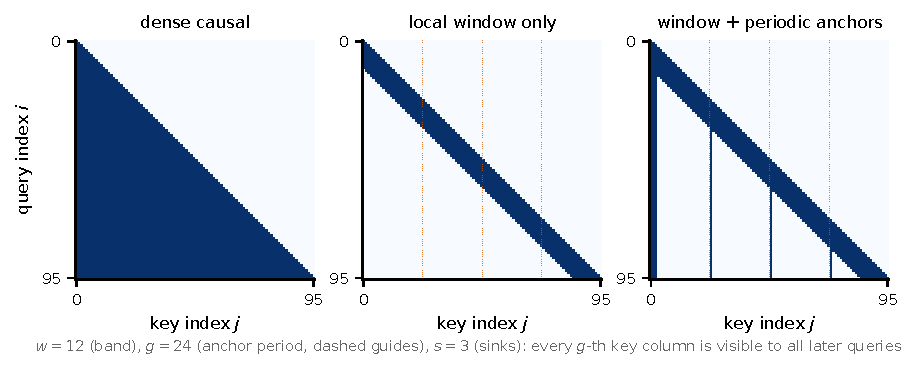
\includegraphics[width=\textwidth]{fig1_mask.pdf}
\caption{The mask family \eqref{eq:mask} at $n=96$, $w=12$, $g=24$, $s=3$. Left:
dense causal attention. Middle: a sliding window, whose global-key budget is zero.
Right: window plus periodic anchors; every $g$-th key column is visible to all
later queries, marked by the dotted guides. The third panel differs from the second
by a set of columns, not by a property of the pattern, and that set is what
Theorem~\ref{thm:linear} counts.}
\label{fig:mask}
\end{figure}

Two readings of \eqref{eq:entryasym} matter. First, the anchor term is
\emph{quadratic} in $n$: the count is $n(w+s)$ plus $(n-w)^2/(2g)$, so a fixed
period $g$ gives $\Theta(n^2)$ entries, scaled down by $1/(2g)$. The often quoted
``$\bigO(n(w+n/g))$'' is therefore linear only in the parameter, not in $n$.
Second, the two terms exchange dominance at
\begin{equation}
n^\ast \;=\; 2g\,(w+s),
\label{eq:crossover}
\end{equation}
which for the settings of Section~\ref{sec:device} is $n^\ast=\CrossoverLen$
(Figure~\ref{fig:mask} illustrates the three patterns; Figure~\ref{fig:counting}
shows the count);
below it the window term dominates and the pattern looks linear, above it the
anchor term does. At the largest length we measure, the anchors already account
for \AnchorShareAtLargestN\% of all entries while the mask retains
\DensityAtLargestN\% of the causal matrix. This is the quantitative reason why a
short benchmark suggests that a periodic-anchor design is cheap and a long one
does not.

\subsection{The linearity criterion}

\begin{theorem}[Linearity criterion]\label{thm:linear}
Consider a mask whose attended entries are a window of width $w$ plus a
global-key set of size $A(n)$ that is visible to all later queries. Then
\begin{equation}
\lvert\Sset\rvert \;=\; n\,(w+s) \;+\; \Theta\!\left(n\,A(n)\right),
\end{equation}
so the cost is $\Theta(n)$ if and only if $A(n)=\bigO(1)$, and $\Theta(n^2)$ if
$A(n)=\Theta(n)$.
\end{theorem}

The argument is a double count: each global key is attended by every later query,
hence contributes $\Theta(n)$ entries, and there are $A(n)$ of them; the window
contributes $nw$. Theorem~\ref{thm:linear} is what separates the two designs that
the literature groups under ``global attention''. A fixed global set costs
$n\lvert G\rvert$, which is linear with a constant that does not grow; a periodic
anchor set costs $n^2/(2g)$, which is quadratic however small the constant looks
at the $n$ where it was benchmarked. It also explains why a learned selection
budget that is constant per query (as in \cite{zhou2021informer}) stays in the
linear class while a coverage-driven period does not.

There is a second, harder consequence. Combining \eqref{eq:entryasym} with
Proposition~\ref{prop:block} below, the work a block-granular kernel actually
performs for the anchor term is $\Theta(n^2 B/(2g))$, i.e. the effective period is
$g/B$ blocks rather than $g$ positions. The achievable reduction relative to
dense attention is therefore bounded by $g/B$, a small constant for the anchor
periods at which the mask is at all faithful
(Corollary~\ref{cor:ceiling}).

\subsection{What a block-granular kernel actually executes}\label{sec:blocklaw}

A kernel does not execute a mask; it executes a set of $B\times B$ tiles. The
executed density is therefore a different random variable from the density of the
mask, and the difference is systematic rather than noisy.

\begin{proposition}[Granularity law]\label{prop:block}
Partition the sequence into blocks of size $B$ and let $D_{\mathrm{blk}}$ be the
fraction of causal key blocks that the pattern requires. Then
\begin{equation}
D_{\mathrm{blk}} \;=\; \min\!\left(1,\frac{B}{g}\right) \;+\; D_{\mathrm{win}},
\label{eq:blocklaw}
\end{equation}
where $D_{\mathrm{win}}$ is the diagonal band contributed by the window, and the
first term does not depend on whether $g$ is a multiple of $B$.
\end{proposition}

The first term is a counting identity: a key block of $B$ consecutive positions
contains a multiple of $g$ whenever $B\ge g$ (pigeonhole, so the term saturates at
one), and otherwise contains one with frequency $B/g$; a block that contains an
anchor is materialised even if the anchor is its only useful entry. Alignment
between $g$ and $B$ moves the anchor to the block boundary, which matters for
addressing in a streaming kernel, but it does not change how many blocks are
needed. Table~\ref{tab:block} checks \eqref{eq:blocklaw} at six settings and the
two sides agree to three decimals in all of them.

The consequence is a multiplicative inflation of the sparse work,
\begin{equation}
\frac{D_{\mathrm{blk}}}{D_{\mathrm{elm}}} \;\approx\; B
\quad\text{for } g>B,
\label{eq:inflation}
\end{equation}
because the element-level anchor density is $1/g$ while the block-level density is
$B/g$. At $B=\AlignBlock$ and $g=192$ the measured inflation is
\BlockInflationAtRef{}$\times$: a mask that is \BlockElemDensPct\% dense at element level
occupies \BlockDensCausalAtB\% of the causal blocks. The factor $B$ in
\eqref{eq:inflation} is an upper envelope, approached only once the window term
has stopped contributing to the element density; at the lengths we can measure it
still contributes, which is why the measured factor is \BlockInflationAtRef{}
rather than \AlignBlock. Equation~\eqref{eq:inflation} is the second number a
designer needs, and it is the one that the phrase ``$0.5\%$ sparse'' hides.

\subsection{The price of a cheaper mask}

Sparsity is not free in quality, and the price can be stated exactly enough to be
checked.

\begin{theorem}[Retained-mass bound]\label{thm:mass}
Let $a_i$ be the dense causal softmax distribution of query $i$, let
$\rho_i=\sum_{j\in\Sset(i)}a_{ij}$ be the mass it places on the retained set, and
let $a^{\Sset}_i$ be the renormalisation of $a_i$ onto $\Sset(i)$. For any value
matrix with $\lVert V\rVert_\infty=V_{\max}$,
\begin{equation}
\big\lVert o_i^{\mathrm{full}} - o_i^{\Sset}\big\rVert_\infty
\;\le\; 2\,(1-\rho_i)\,V_{\max}.
\label{eq:massbound}
\end{equation}
\end{theorem}

The proof is two lines of total-variation (\ref{app:proofs}) but the
bound is useful because both sides are measurable: $\rho_i$ is computable from the
dense softmax, and the left-hand side is computable by running both attention
variants. Section~\ref{sec:mass} reports the check. The theorem also explains why
the efficiency question cannot be settled on the mask alone: a mask that keeps
$16\%$ of the mass has a worst-case output error of $1.68\,V_{\max}$ before any
kernel is involved.

\begin{corollary}[Ceiling on the anchor saving]\label{cor:ceiling}
For the family \eqref{eq:mask} executed at block granularity $B$, the reduction in
attention work relative to dense attention is at most $g/B$, and the mass retained
by the same mask at length $n$ is approximately $(w+s)/n + 1/(2g)$ in count terms.
Since the retained mass decreases in $g$ while the ceiling increases in $g$, the
two objectives are in direct tension and no choice of $g$ improves both.
\end{corollary}

Corollary~\ref{cor:ceiling} is the compact statement of the design problem, and it
is the reason the measurements below come out the way they do: at $g=\GpuG$,
$B=\GpuBlock$ the ceiling is a factor of four, while the mask keeps
\RhoMean{} of the softmax mass. A designer who wants more than a factor of four
must raise $g$, and every increase buys work at the price of fidelity.

\subsection{From laws to testable hypotheses}

The theory yields seven statements, each of which the artefact marks as a
hypothesis that may come out false. They are listed with the experiment that
tests them, and Section~\ref{sec:attention} reports the verdict on each.

\begin{description}\itemsep2pt
\item[H1] Equation~\eqref{eq:entrylaw} matches the measured entry count exactly on
the grid $n\in\{256,\dots,4096\}$. (Table~\ref{tab:counting}.)
\item[H2] The local log-log exponent of $\lvert\Sset\rvert$ rises from one to two
across $n^\ast$, so a benchmark below $n^\ast$ certifies linearity that does not
hold above it. (Figure~\ref{fig:counting}.)
\item[H3] The transient memory of an anchor-based implementation grows
quadratically while the same implementation with the anchors removed grows
linearly. (Figure~\ref{fig:device}.)
\item[H4] On a memory-constrained device the anchor-based implementation is no
better than a fused dense kernel in either memory or latency at large $n$.
\item[H5] The executed block density equals $\min(1,B/g)$ plus the window term at
every measured setting. (Table~\ref{tab:block}.)
\item[H6] The retained mass is small and the bound \eqref{eq:massbound} holds with
slack. (Section~\ref{sec:mass}.)
\item[H7] A half-billion-parameter instruction-tuned model does not approach a
gradient-boosted baseline on the same rows, and adapting it on $10^2$ rows
repairs the output format without repairing discrimination.
(Section~\ref{sec:lang}.)
\end{description}
